\documentclass[conference,a4paper]{IEEEtran}

\usepackage{cite}
\usepackage{booktabs}
\usepackage{graphicx}
\usepackage{microtype}
\usepackage{url}

\title{A Comprehensive Linux PTP Driver for Time-Aware GPIO}

\author{
\IEEEauthorblockN{Ahmad Byagowi}
\IEEEauthorblockA{Time Appliance Project\\
USA\\
ahmad.byagowi@ocproject.net}
\and
\IEEEauthorblockN{Kevin Stanton}
\IEEEauthorblockA{USA\\
kevin.b.stanton@gmail.com}
\and
\IEEEauthorblockN{David J Zage}
\IEEEauthorblockA{Intel Corporation\\
USA\\
zage@cerias.net}
}

\begin{document}

\maketitle

\begin{abstract}
Clock synchronization makes time comparable across systems, but measurement and control applications also need to attach that time to physical signals. Time-Aware GPIO (TGPIO) provides that timed I/O boundary, capturing external edges and generating scheduled output transitions in the platform time domain. This paper presents a Linux driver that exposes firmware-undeclared Intel TGPIO hardware through the standard PTP hardware clock interface. The driver maps known MMIO resources, configures each block for external timestamp input or periodic output, and integrates the Always Running Timer (ART) timebase with Linux timekeeping, offering realtime, raw ART, and adjustable PHC clock modes usable with existing PTP tools. We report output semantics established through register-level experiments (single-shot compares that never fire, an unreadable output level flop, and glitch-free in-flight rewrites of the interval and compare registers) and a discipline design built on them that steers a free-running hardware output without waveform restarts while tracking polarity in software. Measured with a logic analyzer against the atomic-clock-referenced PPS of an OCP TimeCard, the disciplined TGPIO 1~PPS output achieves a mean offset of $+9$~ns with a standard deviation of 64~ns, statistically comparable to the TimeCard's own PPS output on the same instrument. A KMDF driver for the same blocks under Windows, reusing those hardware findings unchanged, shows that the register-level semantics are portable while the clock integration is not. TGPIO can thus turn an otherwise internal PTM/PTP-aware timing domain into usable physical I/O for synchronization, measurement, and control.
\end{abstract}

\begin{IEEEkeywords}
Precision Time Protocol, Precision Time Measurement, Time-Sensitive Networking, PTP hardware clock, timed I/O, Time-Aware GPIO, GPS PPS, ART, Linux kernel
\end{IEEEkeywords}

\section{Introduction}

Precision timing systems often need more than a synchronized network clock. They also need physical I/O that binds external events to a shared timebase: timestamping a pulse-per-second (PPS) signal, measuring an instrument trigger, or generating a scheduled output transition for a device under test. Linux already provides a mature PTP hardware clock (PHC) abstraction for these ancillary functions, including external timestamp input and periodic output generation \cite{linux-ptp-docs}.

A concrete example is a small system that needs accurate time from a GPS receiver but has no network interface card PHC, FPGA, or dedicated timing card. If the receiver's PPS edge can be timestamped directly by TGPIO and exposed as a PHC external timestamp event, linuxptp tooling can discipline the TGPIO PHC and transfer that time to the system clock. This minimal-hardware path from an external time reference into Linux timekeeping also lets the operating system participate in the timing domain of a Time-Sensitive Networking (TSN) system \cite{ieee8021as}.

Some commodity platforms contain timed I/O resources that firmware never enumerates, so standard platform-driver discovery fails even though the underlying MMIO register block is present and functional. The result is an awkward gap: hardware useful for synchronization and measurement that applications have no standard way to reach.

This paper describes an out-of-tree Linux driver that bridges that gap for Intel Time-Aware GPIO (TGPIO) blocks on a tested desktop platform. The driver maps known static MMIO resources, exposes each block as a PTP pin, and allows the block to be configured as an external timestamp input, a periodic output generator, or unused. It is designed around the Linux PHC interface rather than a custom userspace ABI, so existing tools such as \texttt{testptp} work unmodified; a companion Python library, PyPTM, wraps the same public PTP character-device interface for scripted experiments \cite{pyptm-repo}.

The central design problem is not only register access: TGPIO capture and compare values live in the platform ART domain, while the PTP clock interface presents timestamps in a PTP clock domain. The driver therefore defaults to an ART-backed adjustable PHC, provides explicit realtime and raw ART modes for compatibility and diagnostics, and handles bring-up issues that are easy to miss in a purely architectural description, such as input edge defaults, deterministic output startup, and output polarity.

This work contributes a PTP-clock abstraction for static TGPIO MMIO blocks that firmware does not enumerate, with per-block selection of external timestamp input, periodic output, or disabled operation; a timestamp path supporting realtime-converted captures, raw ART-derived timestamps, and a default ART-backed adjustable PHC mode for tools such as \texttt{ts2phc}; experimentally established TGPIO output semantics (toggle-only level state, inert single-shot compares, safe hot register rewrites) and a discipline design built on them, combining grid-aligned re-arms, in-flight interval refresh, sub-100~ns phase nudges, and software-tracked polarity; a one-shot external calibration that cancels constant clock-comparison and pipeline delays, bringing a disciplined 1~PPS output within 100~ns of an atomic reference; and a Windows KMDF port of the same blocks reusing those hardware findings unchanged, which separates what is portable about timed I/O from what each operating system's clock model forces.

\section{Background}

\subsection{Linux PTP Hardware Clocks}

Linux exposes hardware-assisted precision timing through the PHC subsystem: a driver registers a \texttt{struct ptp\_clock\_info}, implements operations such as \texttt{gettime64()} and \texttt{enable()}, and advertises ancillary features that userspace configures through the PTP character device. The key pin functions here are \texttt{PTP\_PF\_EXTTS}, which emits timestamped edge events, and \texttt{PTP\_PF\_PEROUT}, which requests a periodic output \cite{linux-ptp-docs,linux-ptp-header}. This boundary avoids inventing a new control plane and lets existing tools drive TGPIO, with pin assignment selecting the physical block for each function.

\subsection{ART, TSC, and Cross Timestamps}

Modern Intel platforms relate the Time Stamp Counter (TSC), the ART, and system time: CPUID leaf \texttt{0x15} reports a crystal clock frequency and TSC-to-crystal ratio on supported processors \cite{intel-sdm}, and Linux timekeeping exposes cross-timestamp support for relating device counter values to system time \cite{linux-timekeeping-docs,linux-crosststamp-rfc}.

The TGPIO hardware used by this driver captures and compares ART-domain counter values; the driver converts between ART and the active PTP clock domain in both directions, as detailed in Section~IV.

\subsection{Firmware Enumeration Gap}

Upstream and public discussion around Intel timed I/O shows that TGPIO-like facilities have existed in Linux development contexts \cite{linux-pps-gen-tio,lkml-tgpio-pmc,lkml-tgpio-io}, but the platform studied here does not enumerate the relevant ACPI device. The driver therefore takes the MMIO base addresses as platform-specific module parameters, which is less general than firmware discovery but useful when the hardware exists and the address map has been confirmed.

\section{Driver Design}

\subsection{Static Blocks and Module Parameters}

The driver supports two static TGPIO blocks, each with a configurable MMIO base address (defaults \texttt{0xFE001210} and \texttt{0xFE001310}, span \texttt{0x38} bytes) and an independent mode: \texttt{input}, \texttt{output}, or \texttt{off}. The default configuration enables both blocks as rising-edge external timestamp inputs.

Table~\ref{tab:params} summarizes the most relevant module parameters. Keeping platform identity outside the driver binary makes the module easy to test where the MMIO resources are known while avoiding a false claim of general platform discovery.

\begin{table}[t]
\caption{Selected Driver Parameters}
\label{tab:params}
\centering
\footnotesize
\begin{tabular}{@{}p{0.42\linewidth}p{0.14\linewidth}p{0.33\linewidth}@{}}
\toprule
Parameter & Default & Purpose\\
\midrule
\texttt{addr0}, \texttt{addr1} & static & TGPIO MMIO bases\\
\texttt{tgpio0}, \texttt{tgpio1} & input & per-block function\\
\texttt{edge0}, \texttt{edge1} & rising & default input edge\\
\texttt{clock\_mode} & phc & realtime or adjustable PHC\\
\texttt{timestamp\_mode} & realtime & event timestamp domain\\
\texttt{output\_polarity} & normal & logical output polarity\\
\texttt{poll\_ms} & 10 & input polling interval\\
\texttt{art\_frequency} & 0 & ART conversion frequency\\
\texttt{output\_phase\_offset\_ns} & 0 & output edge calibration\\
\bottomrule
\end{tabular}
\end{table}

\subsection{PTP Pin Model}

At load time, the driver maps all enabled blocks and registers a single PTP clock, with each block becoming a PTP pin descriptor named by its physical index and mode. Pin verification accepts external timestamp requests only on input-mode blocks and periodic-output requests only on output-mode blocks. Channel mapping follows the PTP pin assignment model (\texttt{testptp -L}); absent an explicit assignment, the driver falls back to a direct channel-to-block mapping.

\subsection{Userspace Control}

The primary control surface is the standard PTP character device, not a private ABI: \texttt{testptp} covers pin assignment, external timestamp enablement, and periodic-output requests, and PyPTM provides the same operations as a Python API. One compatibility detail is worth recording: recent kernels validate the strict \texttt{PTP\_EXTTS\_REQUEST2} ioctl's flags against the \texttt{supported\_extts\_flags} field of \texttt{ptp\_clock\_info} before the driver sees the request, so a driver leaving that field zero silently rejects every strict request while the legacy ioctl still succeeds. Advertising the supported flags fixed \texttt{ts2phc}, and is worth checking in any PHC driver that predates the field.

\subsection{External Timestamp Input}

For input mode, enabling a PTP external timestamp request configures the block for input, applies the edge selection, and starts a poll worker that reads the capture timestamp and event counter. The register sequence matters: reading the low capture timestamp register latches the associated timestamp and event-count values before the remaining registers are read.

When the event count changes, the driver emits a PTP external timestamp event through the PHC event path, timestamped according to the selected timestamp mode (a debug option can substitute the poll time). Captures also feed ancillary consumers: per-input phase and interval statistics in the status file, an RFC~2783 PPS source per input block for NTP-family tools, and a time-to-digital converter mode that pairs start and stop captures across the two blocks with one-ART-cycle resolution. The PHC additionally implements precise cross-timestamps (\texttt{PTP\_SYS\_OFFSET\_PRECISE}), which \texttt{phc2sys} and chrony adopt automatically.

\subsection{Periodic Output}

For output mode, a PTP periodic-output request supplies a start time and period in the PTP clock's time domain. The driver rejects unsupported perout flags, validates the period, computes a half-period, and requires that Linux timekeeping expose an ART base clock. It then converts the requested start time into an ART compare value and the requested half-period into an ART interval value before programming the hardware.

Steady-state output uses the TGPIO hardware periodic feature: the comparator holds the first active edge, the interval register holds the half-period in ART cycles, and the periodic-mode bit lets hardware generate subsequent toggles without per-edge software work. Register-level experiments established that single-shot output compares never fire on this hardware and that the output level flop is write-only toggle history: it holds the last generated level, survives disable, and cannot be preloaded or read back. The driver therefore mirrors the flop in software: it assumes the power-on low state at load, folds every generated toggle into the mirror via the live comparator readback, drains the flop low before stops and unloads so the assumption survives reloads, and selects the first compare slot so rising edges always land on the requested period grid. A guard pushes a late first compare forward by whole periods (a compare already in the past fires immediately and would invert the waveform), and a debugfs control flips the mirror if interference ever falsifies it, shifting a running waveform by half a period without a glitch. The same engine serves asymmetric duty cycles whose halves are both at least 50~ms by alternating the interval register between on-time and off-time counts (a 25\% duty request measured 249.998~ms/749.995~ms) and provides hardware-timed one-shot pulses; an hrtimer path remains for narrower pulses. One negative result is worth recording: with a 50\% duty output, edge timestamps alone cannot distinguish rising from falling edges, so polarity is unobservable from an external reference, becoming observable (and self-correcting) only in a loopback configuration where an input captures the output's own rising edges.

Quantization is reported, not hidden: converting a request onto integer ART cycles rounds both the half-period and the first edge (each bounded by half a 26~ns cycle at the 38.4~MHz ART rate), and every arm logs both residuals, the first-edge one measured by reading the programmed compare value back through the clock conversion. The debugfs status file exposes the same quantities continuously, with the live phase error of the pending edge and the tracked output level.

\section{Clock-Domain Handling}

The driver supports three PTP clock modes; internally, the TGPIO registers always use ART-domain counter values for both capture and compare. The default mode exposes an ART-backed adjustable PHC with \texttt{settime64()}, \texttt{adjtime()}, and \texttt{adjfine()} support, so a GPS PPS signal connected directly to a TGPIO input can become the external reference for tools such as \texttt{ts2phc}, after which other Linux time tools can make the disciplined time available to the system. An \texttt{art} mode reuses the same anchor-plus-rate clock model but rejects every adjustment, providing an undisciplined hardware-paced timebase; calibrating its rate against \texttt{CLOCK\_MONOTONIC\_RAW} can only recover the nominal ratio (that clock shares ART's crystal, so the crystal's ppm-scale error remains), while an alternative realtime calibration tracks the kernel timekeeper's rate with a sliding-window estimator and a runtime trim accepts an operator calibration from an external instrument.

An explicit realtime mode ties \texttt{gettime64()} to \texttt{CLOCK\_REALTIME} and maps the PTP adjustment operations onto the system clock itself. Because that clock is also steered behind the driver's back (chrony, \texttt{adjtimex}), realtime-mode outputs are re-synchronized to the realtime grid once per second using the same glitch-free nudge machinery as PHC mode. A reference pulse captured by a TGPIO input can then discipline the operating-system clock directly from hardware timestamps; validated with a chrony PHC-refclock configuration, the system clock locked to the atomic PPS with a $-218$~ns offset and 11~ns per-sample standard deviation. In a TSN deployment this gives the OS a local disciplined timebase for host-side timestamping and scheduling; network transmission still depends on the NIC and TSN stack.

For input events in realtime mode, the driver constructs a device cross-timestamp context from the captured ART cycle count and the Linux ART clocksource identifier, calls the kernel cross-timestamp interface, and uses the returned realtime value as the event timestamp; in PHC mode, captured cycles are converted into the adjusted PHC domain by applying the current offset and frequency scale. The raw ART mode converts cycles to nanoseconds using the configured or CPUID-detected frequency, which is useful for debugging the counter scale but claims no realtime epoch alignment.

For output events, the userspace request is expressed in the PTP clock domain while the hardware compare and interval registers expect ART cycles. Realtime mode converts through Linux timekeeping's realtime-to-ART relationship; PHC mode uses the driver's stable ART base rate plus the adjusted PHC offset and frequency scale; the periodic interval register uses the same conversion. If the required relationship or base rate is unavailable, the driver fails the request rather than scheduling an edge in the wrong domain.

A running hardware output must also follow PHC discipline. The PHC base rate is calibrated from the kernel timekeeper at load, since the nominal CPUID crystal frequency differs from the effective rate by tens of ppm on the tested platform. A PHC step re-arms the output with the first edge advanced along the originally requested period grid, so a step never shifts the waveform phase. A frequency adjustment rewrites the periodic interval register in flight (such writes latch cleanly for subsequent periods), and residual phase errors above 50~ns, measured against the pending edge read live from the comparator, are corrected by rewriting the comparator, which moves only the pending edge and produces no glitch. Finally, a runtime-writable calibration offset shifts every programmed edge by a constant, letting a one-shot external measurement cancel systematic delays such as the asymmetric PCIe read latency in PHC-to-PHC comparison.

\section{Bring-Up Lessons}

Several implementation details emerged only during bring-up. First, the input default was changed to rising edge: both-edge capture doubles the apparent event rate and rarely matches PPS or trigger workflows.

Second, the modes need different dependency checks: raw ART conversion and hardware periodic intervals require an ART frequency value (supplied or CPUID-detected), while realtime conversion relies on Linux timekeeping's ART base-clock relationship; the driver reports the CPUID values for diagnostics either way.

Third, the output semantics above differed substantially from the initial mental model and were settled only by direct register experiments observed with a logic analyzer: an initially implemented ``preconditioning edge'' relied on single-shot compares and was a silent no-op, the edge-polarity field has no effect on outputs, and no register round-trip reveals the output level. An earlier belief that in-flight register rewrites corrupt the waveform originated from an older driver revision and dissolved under controlled experiments; the one real caveat is that a comparator rewrite can register a phantom event that flips the level-mirror parity, so the driver pauses the periodic-mode bit around such rewrites while output enable holds the line level. Because the analyzer captures were scripted, each wrong hypothesis was falsifiable within minutes; this loop of poke, capture, and decode was the single most productive bring-up tool.

\section{Evaluation}

The tested platform is an ASUS ProArt Z890-CREATOR WIFI motherboard (BIOS 3202) running Ubuntu 26.04 LTS with Linux \texttt{7.0.0-27-generic}, using the default addresses and two-block setup. The reference is an OCP TimeCard whose PHC (\texttt{ptp\_ocp}) is fed by its onboard atomic clock. A Saleae Logic Pro 16 samples four channels at 100~MS/s (10~ns resolution), observing the atomic 1~PPS, the TimeCard PPS, and both TGPIO outputs; the analyzer's crystal error cancels because all results are channel-to-channel differences against the atomic PPS. \texttt{phc2sys} disciplines the TGPIO PHC from the TimeCard PHC at eight updates per second.

\begin{table*}[t]
\caption{Measured 1~PPS Output Performance (100~MS/s logic analyzer, atomic-clock PPS reference)}
\label{tab:eval}
\centering
\footnotesize
\begin{tabular}{@{}p{0.25\textwidth}lllp{0.23\textwidth}@{}}
\toprule
Configuration & Rate error & Mean offset & Std.\ dev. & Notes\\
\midrule
Free running (PHC anchored to \texttt{CLOCK\_REALTIME}) & $-28.4$~ppm & --- & --- & tracks system clock, by design\\
Disciplined, before calibration & $<0.001$~ppm & $+2.38$~$\mu$s & 52~ns & constant PHC-comparison asymmetry\\
Disciplined, after one-shot calibration & $<0.001$~ppm & $+9$~ns & 64~ns & 180 pulses\\
TimeCard PHC PPS (reference hardware) & $<0.001$~ppm & $-10$~ns & 54~ns & same instrument and reference\\
\midrule
ART mode, raw calibration & $-41$~ppm & --- & --- & same-crystal calibration; crystal error retained\\
ART mode, realtime calibration & tens of ppb & free-running phase & --- & sliding-window rate from the disciplined system clock\\
Realtime mode, gentle system servo & tracks system clock & within $\pm 150$~ns of atomic & --- & 1~Hz PI \texttt{phc2sys} to a PTM master; 1~s output re-sync\\
Realtime mode, aggressive system servo & tracks system clock & $\pm 250$~ns band & --- & 8~Hz linreg servo dither reproduced at the pin\\
\bottomrule
\end{tabular}
\end{table*}

Table~\ref{tab:eval} summarizes the output results. Once \texttt{phc2sys} locks the TGPIO PHC to the TimeCard, the interval-refresh path removes the rate error entirely: over two-minute captures the mean period matches the atomic reference at the instrument's resolution, with zero waveform restarts and driver-reported phase error below 100~ns. The residual $+2.38$~$\mu$s offset before calibration is constant (drift below 1~ns/s) and dominated by asymmetry in the PHC-to-PHC comparison: reading the TimeCard PHC across PCIe costs several microseconds round trip while the TGPIO read is a fast timekeeping conversion, and \texttt{phc2sys} assumes symmetric readings. Writing the measured constant into the calibration parameter moves the output to $+9 \pm 64$~ns, statistically comparable to the TimeCard's own PPS on the same instrument ($-10 \pm 54$~ns); the remaining spread is consistent with the 26~ns ART quantization step plus servo wander. Reaching this floor also required pinning the platform (\texttt{/dev/cpu\_dma\_latency} at zero, performance cpufreq governor) to stabilize the PCIe read latency, and the constant must be recalibrated if that regime changes.

Polarity determinism was validated separately: across five module reloads, deliberate 300~ms PHC steps, and \texttt{phc2sys} restarts, both outputs came up with rising edges on the requested grid every time, and a falsified level mirror was corrected through the debugfs control while running, snapping the inverted waveform onto the grid without a glitch.

The hardware-domain loop was then closed: the reference PPS was wired into a TGPIO input and \texttt{ts2phc} disciplined the PHC from that block's own ART-domain timestamps, with the second block generating the output. Capture and generation share the ART timebase, so the PCIe comparison drops out entirely: the uncalibrated offset collapses from $2.4$~$\mu$s to about $+50$~ns (roughly two ART cycles of pipeline difference), with no latency pinning required. Alignment measured $-52 \pm 122$~ns against a reference whose own wire-to-wire noise floor was 60--80~ns. Both discipline paths therefore land within about $\pm 100$~ns of the atomic reference, the input-capture path being preferable because its systematic error needs no external calibration. This configuration is the complete GPS use case with the atomic PPS standing in for a receiver.

\begin{figure}[t]
\centering
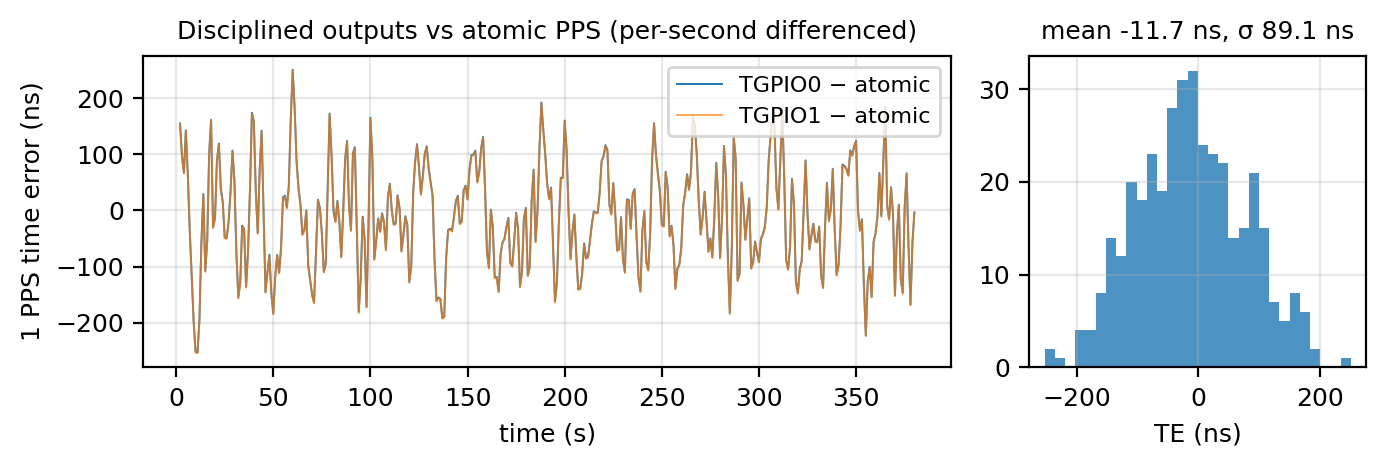
\includegraphics[width=0.92\columnwidth]{figures/commonview-te.png}\\[0.3em]
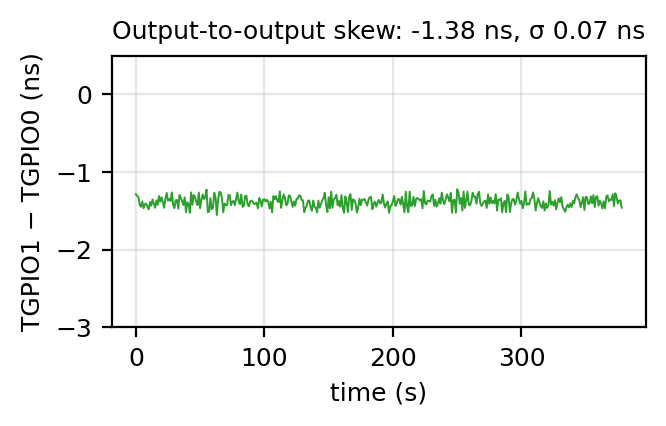
\includegraphics[width=0.62\columnwidth]{figures/dual-output-skew.png}
\caption{Sentinel common-view measurement of both disciplined TGPIO 1~PPS
outputs, differenced per second against the atomic reference channel to
cancel the instrument timebase. Top: time series over the calibrated window
and the TGPIO0 error distribution ($-12 \pm 89$~ns; the spread combines the
two channels' trigger noise in quadrature). Bottom: output-to-output skew
from the same window, a constant $-1.4$~ns (cable length) with 0.07~ns
standard deviation.}
\label{fig:commonview}
\end{figure}

The output path was cross-validated on an independent instrument. A Calnex Sentinel measured 1~PPS time error simultaneously on both TGPIO outputs and on the atomic reference, differencing per second against the reference channel to cancel the instrument's free-running timebase. With both blocks disciplined through the phc2sys path, a 15-minute run measured $-42 \pm 103$~ns and a 7-minute run $-66 \pm 83$~ns, with residual drift below $0.25$~ns/s; repeated windows show the PCIe-path systematic wandering on a $\pm 60$~ns scale over tens of minutes, which bounds how finely the delay calibration is worth trimming. The two outputs tracked each other at $-1.4 \pm 0.1$~ns (Fig.~\ref{fig:commonview}), so a second synchronized hardware output costs nothing in accuracy.

\begin{figure*}[t]
\centering
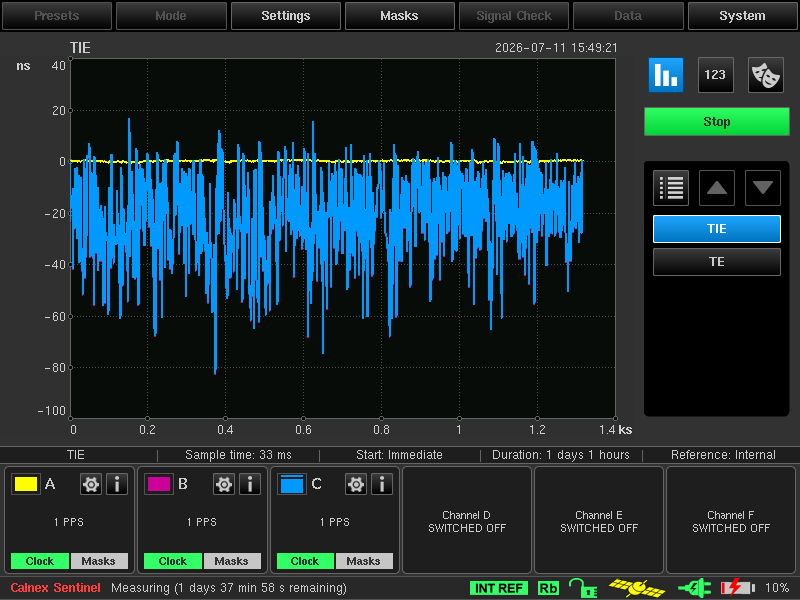
\includegraphics[height=3.3cm]{figures/sentinel-ptm-run.png}\hspace{1.5em}
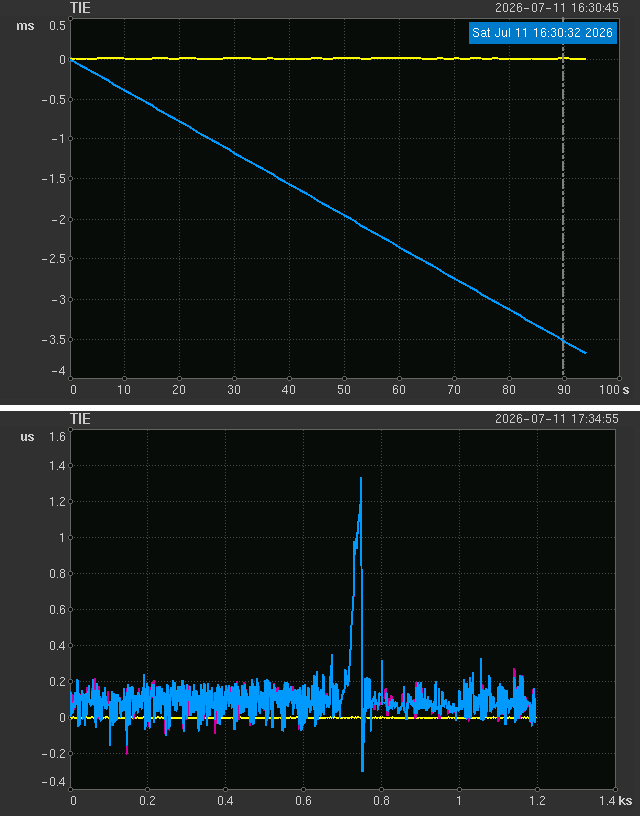
\includegraphics[height=3.3cm]{figures/clock-mode-calibration.png}
\caption{Instrument displays. Left: the PTM-era run, 1.4~ks of TIE with the
PTM-disciplined chain and zero delay calibration; the master card's own PPS
(flat trace) and the TGPIO output (band) stay within tens of nanoseconds of
the shared atomic reference. Right pair: clock-mode calibration. ART mode
with raw calibration drifts at $-41$~$\mu$s/s (the crystal's own error),
while realtime mode with a gently disciplined system clock (1~Hz PI
\texttt{phc2sys} from the PTM master) and one-second output re-sync holds the
atomic-aligned realtime grid within roughly $\pm 150$~ns; the single
transient marks the servo restart itself.}
\label{fig:ptmrun}
\end{figure*}

The alternate clock modes were characterized in the same setup (Fig.~\ref{fig:ptmrun}, right). ART mode with the default same-crystal calibration drifts at the crystal error ($-41$~$\mu$s/s measured); with realtime calibration the sliding-window estimator holds the residual rate to tens of ppb, and the operator trim removes the remainder after one instrument measurement. Realtime-mode outputs track the system clock faithfully, so the quality of that clock's discipline dominates: an aggressive 8~Hz linreg \texttt{phc2sys} dithers the frequency and widens the output band to $\pm 250$~ns, while a 1~Hz PI servo against the PTM master holds the pin within about $\pm 150$~ns of the atomic-aligned grid.

Finally, enabling PCIe Precision Time Measurement on the master card (hardware cross-timestamps through \texttt{PTP\_SYS\_OFFSET\_PRECISE}) removed the software-bracketed read asymmetry from the phc2sys comparison entirely: both legs then rest on hardware-paired timestamps, the microsecond-scale delay calibration becomes unnecessary, and a 22-minute common-view run with zero calibration showed smoothed output phase wander of about 10~ns RMS against the shared atomic reference with drift below $10^{-11}$ (Fig.~\ref{fig:ptmrun}). Tightening the driver's phase-nudge dead-band from its 200~ns default to 30~ns and deepening the phc2sys per-sample read filtering reduced each output's absolute spread from 78~ns to 47~ns (below the 69~ns spread of the atomic reference channel itself on the same instrument), with residual drift of $2$~ps/s.

\section{A Windows Counterpart}

The register-level semantics of Section~V are properties of the device, not of Linux, so they should transfer to any operating system able to map the same MMIO. The same two blocks were therefore brought up under Windows as a KMDF driver, which both tests that claim and serves users of the tested platform who do not run Linux. The driver is a root-enumerated software device, the direct analogue of the Linux module's static addressing: firmware enumerates nothing, so it claims no PnP resources and maps the physical addresses itself through \texttt{MmMapIoSpaceEx}. Addresses, MMIO span, block count, and ART frequency live in the service registry key, seeded by the INF with the same defaults as Table~\ref{tab:params}.

The control plane is where the ports diverge, and the divergence is forced. Windows has no PHC abstraction, hence no clock device for \texttt{ts2phc} or \texttt{phc2sys} to bind to and no pin-function model. The driver instead exposes eight buffered IOCTLs (info and block status, cross-timestamp, input enable, capture read, output start, stop, and invert) through one sequential queue, with a command-line tool over them; capture delivery is pull-only, the poll loop living in user mode. Timebase handling degrades similarly. Linux hands captured ART cycles to the timekeeper as a correlated counter and refines the base rate at runtime; lacking any such interface, the Windows driver brackets a \texttt{KeQuerySystemTimePrecise()} read between two \texttt{RDTSC} samples at \texttt{DISPATCH\_LEVEL}, converts the midpoint through the CPUID leaf \texttt{0x15} ratio and the \texttt{IA32\_TSC\_ADJUST} offset, and returns the bracket width so callers can bound the pairing error. That rate is nominal and never refined, so a Windows output free-runs at the crystal's ppm error: the same limitation as the Linux ART mode, but the only option rather than one of three.

What transfers intact is the output engine. The Windows driver arms the same toggle-mode hardware periodic output, applies the same whole-period late-arm guard, mirrors the same unreadable level flop by folding the live comparator readback, and performs the same paused comparator rewrite for a glitch-free half-period inversion. That code was written directly from Section~V's findings and worked without further hardware archaeology, the strongest available evidence that those findings describe the device rather than the driver. The port also enabled a useful testing technique: a host-side harness compiles the unmodified driver sources against stub headers on an ordinary POSIX toolchain, replacing the register accessors with a logging shim, so assertions can check the programming \emph{sequence} (interval before comparator before the enabling control write, enable asserted exactly once, the pause bracket around an inversion) rather than final state alone. Ordering is precisely what this hardware is sensitive to, and the tests run in a second with no kernel, target machine, or analyzer.

Several Linux features are not ported: no disciplining or servo, no PPS source, no asymmetric duty cycle or one-shot pulse, and no automatic polarity recovery. The driver generates a UTC-aligned 1~Hz output on the tested platform, but the measurement campaign has not been repeated there, and every number reported in this paper is from Linux.

\section{Limitations and Future Work}

The current implementation is intentionally platform-specific: it requires known MMIO addresses and should only be loaded where those have been confirmed. A production-quality upstream driver would need robust platform discovery, ownership checks, and maintainable quirks. The external timestamp path is polling-based, which keeps the driver compact but creates a latency and event-loss tradeoff controlled by \texttt{poll\_ms}; an interrupt-backed path would be preferable for high-rate streams. The default PHC mode adjusts a software clock model layered on ART rather than disciplining the ART oscillator itself, unlike a NIC PHC that owns an independent hardware clock.

Output polarity ultimately rests on one bit of external truth: the level flop cannot be read, so anything toggling the pin outside the driver requires a one-shot external observation to correct through the debugfs flip control. Tools holding the PTP character device open must also be restarted after a module reload, because the clock device is recreated.

Future work includes the remaining timestamp-mode comparisons, repeating the measurement campaign on the Windows port, validating additional platforms, replacing static addressing with a discovery or quirk mechanism, adding interrupt support where available, and evaluating whether a subset of the design is suitable for upstream Linux review.

\section{Conclusion}

This work shows that firmware-undeclared timed I/O hardware can be made useful through the standard Linux PTP interface: presenting each mapped TGPIO block as a PTP pin lets existing tools control hardware that would otherwise be unreachable, and a direct TGPIO input provides a compact path from an external time reference into host timekeeping.

The decisive engineering issues are clock-domain correctness and deterministic output behavior, addressed with explicit timestamp modes, cross-timestamp conversion, realtime-to-ART scheduling, and a software mirror of the write-only level state. With in-flight interval refresh, live comparator phase nudges, and a one-shot delay calibration, a disciplined TGPIO output holds an external atomic PPS reference within 100~ns, comparable to a dedicated timing card's own output. The Windows port reinforces the division of labor: the hardware semantics carried over unchanged, while the clock integration had to be rebuilt around what that operating system exposes.

\section*{Availability}

Both drivers, build tooling, measurement scripts, and documentation are
available at \url{https://github.com/ahmadexp/TGPIO} under the TGPIO
Non-Commercial License; commercial use requires written permission. The Linux
module's GPL-compatible \texttt{MODULE\_LICENSE} string exists solely to
satisfy the kernel's licensed-symbol requirements.

\section*{Acknowledgment}

The authors would like to thank the people in Asus and AMI who supported the implementation of various pieces needed for this work to become a reality.

\bibliographystyle{IEEEtran}
\bibliography{references}

\end{document}
